% Modalités:
% 20 pages max (y compris biblio)
% deadline: 27 mars 2018, 13h

% Plan:
% 1 - Contexte, positionnement et objectif de la proposition :
%   Décrire les objectifs et les hypothèses scientifiques. Montrer l’originalité et la pertinence
%   par rapport à l’état de l’art. Décrire la méthodologie et la gestion des risques
%   scientifiques.
% 2 - Organisation du projet et moyens mis en œuvre :
%   Présenter le coordinateur scientifique et son implication. Présenter le consortium et sa
%   complémentarité. Détailler le programme de travail et la répartition des tâches entre les
%   différents partenaires, illustrer par un diagramme de Gantt. Décrire les moyens mis en
%   œuvre pour atteindre les objectifs (devront notamment apparaître : la justification des
%   moyens demandés par postes de dépenses et en lien avec les objectifs, le contexte en
%   terme de moyens humains et financiers du projet au regard notamment d’autres projets
%   en cours).
% 3 - Impact et retombées du projet :
%   Décrire dans quel(s) domaine(s) (scientifique, économique, social ou culturel) les
%   résultats du projet peuvent avoir un impact. Décrire en quoi les attendus du projet
%   répondent aux enjeux de recherche inscrits au Plan d’Action 2018 de l’ANR. Décrire la
%   stratégie de diffusion et/ou de valorisation envisagée.
% 4 - Bibliographie :
%   En absence d’annexe, la bibliographie doit être contenue dans le document scientifique
%   à soumettre.


% Ne pas mettre de tilde (~), mais un blanc, avant \cite

% Il est recommandé d’utiliser une mise en page permettant une lecture
% confortable du document (page A4, times 11 ou équivalent, interligne
% simple, marges 2 cm ou plus, numérotation des pages).

\documentclass[a4paper,11pt,defblank]{article}
%\usepackage{times}
\usepackage{fullpage}
\usepackage[utf8]{inputenc}
\usepackage[T1]{fontenc}
\usepackage{tabularx}
    \newcolumntype{L}{>{\raggedright\arraybackslash}X}
\usepackage[obeyspaces]{url} \urlstyle{sf} %% URLs 
\usepackage{setspace}
\usepackage{titlesec}
\usepackage[dvipsnames,table]{xcolor}
\usepackage{makecell}
\usepackage{multicol}
\usepackage{multirow}
%\usepackage{bibtopic}
\usepackage{eurosym}
\usepackage{calc}
\usepackage{cite}
\usepackage{paralist, tabularx}
\usepackage{wrapfig}
\usepackage{graphicx}
\usepackage{ifthen}
\usepackage{amsfonts,amsmath} %% Additional math chars
\usepackage[nottoc,notlot,notlof]{tocbibind}
\usepackage{paralist} % inline lists 
\usepackage{hhline}
\usepackage{dashrule}
\usepackage{arydshln}
\usepackage{xspace}
\usepackage{float}
\usepackage{pifont}
\usepackage[light,math]{iwona}
\hyphenation{In-ves-tis-se-ment In-volve-ment}
\usepackage[pdftex,                %
  bookmarks         = true,          % Signets
  bookmarksnumbered = true,%     % Signets numérotés
  pdfstartview      = FitH,%     % La page prend toute la largeur
  pdfpagelayout     = SinglePage,% Vue par page
  colorlinks        = true,%     % Liens en couleur
  urlcolor          = blue,%     % Couleur des liens externes
  citecolor         = Blue,
  linkcolor         = Blue,
  pdfborder         = {0 0 0}%   % Style de bordure : ici, pas de bordure
]{hyperref}%                   % Utilisation de HyperTeX 

\setlength{\parskip}{1.2ex plus .4ex minus .4ex}
\setlength{\parindent}{0pt}
\setlength{\parindent}{0pt}

\titleformat{\section} % command
  [hang]     % shape
  {\normalfont\centering\large\scshape\bfseries\color{Blue}} % format Plum
  {\thesection} % label
  {1em} % sep
  {\vspace{-3mm}} % before
  [\vspace{0ex}\titlerule] % after
\titlespacing*{\section}{0em}{0.5em}{0.3em}

\titleformat{\subsection} % command
  [hang]     % shape
  {\normalfont\large\bfseries\color{Mahogany}} % format
  {\thesubsection} % label
  {1em} % sep
  {} % before
  [\titlerule] % after
\titlespacing*{\subsection}{0em}{0.4em}{0.2em}

\titleformat{\subsubsection} % command
  [hang]     % shape
  {\normalfont\bfseries\color{NavyBlue}} % format NavyBlue
  {\thesubsubsection} % label
  {0em} % sep
  {\vspace{-7mm}} % before
  [\titlerule\vspace{-2mm}] % after

\renewcommand{\thesection}{\Roman{section}.}
\renewcommand{\thesubsection}{\thesection\arabic{subsection}.}
\renewcommand{\thesubsubsection}{}

\newboolean{showinstructions}
%\setboolean{showinstructions}{true}
\setboolean{showinstructions}{false} 

\ifthenelse{\boolean{showinstructions}}
 { \newcommand{\instructions}[1]{
        {\noindent\fbox{\parbox{\linewidth-2\fboxrule-2\fboxsep}{#1}}}}}
 { \newcommand{\instructions}[1]{}}

\newboolean{showcomments}
%\setboolean{showcomments}{true}
\setboolean{showcomments}{false}

\ifthenelse{\boolean{showcomments}}
           { \newcommand{\mynote}[2]{
               \fbox{\color{Red}\bfseries\sffamily\scriptsize#1}
               %{\small\emph{\color{Tan}#2}}}}
                    {\small\sffamily{\color{Tan}#2}}}}
           { \newcommand{\mynote}[2]{}}

\newcommand{\todo}[1]{\mynote{TODO}{#1}}
\newcommand{\warning}[1]{\mynote{WARNING}{\textbf{#1}}}

\newcommand{\telecom}[1]{\mynote{Telecom}{#1}}
\newcommand{\pname}{\textsc{Pythia}\xspace}

\newcommand{\francois}[1]{Fran{\c c}ois \textsc{Trahay}{#1}\xspace}
\newcommand{\gael}[1]{Gaël \textsc{Thomas}{#1}\xspace}


\newcommand{\task}{\cellcolor{NavyBlue}\xspace}
\newcommand{\progress}{\cellcolor{Green}\xspace}
\newcommand{\delsoft}{\ding{74}\xspace}
\newcommand{\delreport}{\ding{45}\xspace}
\newcommand{\delexpense}{\ding{80}\xspace}
\begin{document}

\setcounter{secnumdepth}{0}

% feedback
% oracle
% framework
% runtime strategy
\begin{center}

  {\Large\sc\bf\color{Brown}
    \pname: runtime decisions based on prediction (duration: 36 months)
  }\\

%  \vspace{0.4cm}

  {
    \footnotesize
    \pname -- Common 2018 ANR call - JCJC (Jeunes chercheuses/Jeunes chercheurs)\\
    Défi 7 -- Axe 2: Sciences et technologies logicielles\\
  }
  François \textsc{Trahay} -- Télécom SudParis
\end{center}

% The ToC is explicitly required in the specification            
%\setcounter{secnumdepth}{3}
\setcounter{tocdepth}{3}
\tableofcontents

\textbf{Abstract}

Runtime systems have to take decisions that are critical for the
performances of parallel applications. Unfortunately, these decisions
can only use heuristics based on the current status of the application
in order to estimate how it will behave in the future.
%
As a consequence, runtime systems may take decisions that degrade
performances instead of improving them.

\pname aims at providing runtime systems with means to accurately
predict the future. For this, \pname relies on the deterministic
nature of most parallel applications: most programs will behave
similarly from one run to another. Thus, we will design a tool-chain
that analyzes the execution of a program and provides hints to the
runtime systems during future executions of the same program. Thanks
to these hints, a runtime system could base its decisions on both the
current status of the application, and the future behavior of the
program.


\textbf{Evolutions as compared to the first-round proposal}\\

The current proposition is in line with the pre-proposition on the
research directions considered. However, we made some modifications in
order to take into account the evaluations. Specifically, we have
extended the international and national collaborations as part of the
project:

\begin{itemize}
\item A collaboration has been initiated with an international partner
  (University of Chongquing, China). We intend to involve them in
  \pname as part of one of the Tasks. As a result, the travel budget
  has been increased to take into account this collaboration.

\item A recent collaboration with national partners from CEA and INSA
  Lyon has been initiated. We plan to continue this work as part of
  \pname. As a result, we integrated this collaboration in one of the
  planned Tasks.

\item François \textsc{Trahay} recently initiated a collaboration with
  industrial partners in France as part of a proposal for a FUI
  project. Due to his participation in this FUI, François \textsc{Trahay} will now
  invest 66 \% of this time (24p.m) instead of the 80 \% that were
  previously planned. However, we expect that the results of \pname
  could be transferred to industrial partners as part of another FUI
  project.
\end{itemize}

\textbf{Summary of people involved in the project}
\begin{center}
%  \begin{scriptsize}
 \begin{tabularx}{\linewidth} {|p{17mm}|c|p{30mm}|c|L|}\hline
   Partner& Name & Position & Involvement & Role\\\hline Télécom SudParis
   & François \textsc{Trahay} & Associate professor & 24 p.m (66 \%) &
   Project leader: he will ensure that everything goes according to the
   plan. He will co-supervise the PhD student.\\\hline

    Télécom SudParis& Gaël \textsc{Thomas} & Professor& 3 p.m &He will
    help supervising the PhD student.\\\hline

    Télécom SudParis& \emph{To be hired} & PhD student funded by ANR &
    36 p.m & He/she will work on the oracle library and runtime
    systems \\\hline

    Télécom SudParis& \emph{To be hired} & Research intern funded by
    ANR & 6 p.m &He/she will design thread scheduling
    strategies\\\hline

    Télécom SudParis& \emph{To be hired} & Research intern funded by ANR& 6 p.m
    & He/she will help running experiment and contribute to the
    project valorisation\\\hline
 \end{tabularx}
%\end{scriptsize}
\end{center}



\section{Context, positioning and objectives}
% I. Contexte, positionnement et objectif(s) de la proposition

High performance computing has become the
cornerstone of many scientific fields ranging from medical research
to climatology.
%
Efficiently exploiting a supercomputer is difficult. In addition to
expressing the parallelism of an application, it is necessary to
manage the hardware resources of the machine. The way an application
uses the hardware resources may have a significant impact on the
performance: for instance, allocating memory correctly may improve an
application execution time by up to 3.6x relative the default allocation
strategy \cite{carrefour}.

Runtime systems take the responsibility of exploiting the hardware in
place of the program developer by providing an interface to the
application. The task of defining efficient strategies for a
particular hardware setting thus falls to the runtime, and the
application developer can focus on algorithmic.
%
When selecting a strategy, runtime systems analyze how the application
behaved in the past in order to predict how it will behave in the
future.
%
For example, some I/O libraries analyze the data read requests of an
application in order to read the next blocks of data in advance and to
improve the performance of I/O operations \cite{cao1996implementation,
  ding2007diskseen}.

However, the runtime only reacts to the application instead of
anticipating its behavior. This leads to multiple problems as some
early decisions may conflict with later ones. For instance, the
location where memory is initially allocated has a significant impact
on further memory operations and the overhead of moving a memory page
closer to a thread is significant for the application performance
\cite{broquedis2009dynamic}. Reacting to the application is also a
problem for irregular applications where predicting the future
behavior based on past event is difficult.

On the other hand, years of research on performance analysis have led
to many tools that are able to analyze an application behavior and to
identify probable causes of bad performance \cite{hpctoolkit,
  geimer2006scalable, kojak}. Because performance analysis tools
collect various information during a program execution, and analyze
them \emph{post-mortem}, the cost of analysis can be high, whereas a
runtime system has to act quickly in order to reduce its impact on the
performance of the application.  Thus, performance analysis tools can
detect many types of problems ranging from lock contention
\cite{lock_contention}, to inefficient MPI communication patterns
\cite{scalasca}. However, the task of fixing the performance problem
remains the responsibility of the developer.

In this project, we propose to bridge the gap between performance
analysis tools and runtime systems in order to reduce the burden on
the developer. \pname aims at providing runtime systems with
information extracted by performance analysis that would help runtime
system take decisions.

\subsection{Positioning}
% Montrer le caractère novateur du projet, son originalité et le progrès
% qu’il représente par rapport à l’état de l’art ; faire apparaître les
% contributions éventuelles des partenaires du projet à cet état de
% l’art; mentionner d’éventuels résultats préliminaires; dans le cas
% d’une proposition s’inscrivant dans la continuité de projet(s)
% antérieur(s) déjà financé(s) par l’ANR ou par un autre organisme,
% fournir un bilan des résultats obtenus et décrire clairement les
% nouvelles problématiques posées et les nouveaux objectifs fixés au
% regard du/des projets antérieurs.

\vspace{1cm}
\subsubsection{Using performance analysis to improve the performance}
In order to improve the performance of parallel application,
developers need to understand the current performance of their
applications and to detect the causes of performance
degradation. Performance analysis has been studied for a long time, and
many tools for helping developers have been proposed. Many profiling
tools \cite{gprof, linux_perf, arm_map, profiling_mpi} allow users to
spot the hot functions of an application. This information can be used
by developer to identify the functions that are worth
optimizing. Another class of tools consists in generating trace files
depicting an application execution \cite{vampirtrace, eztrace,
  pablo}. User can then navigate through the trace files using
visualization tools \cite{jumpshot, vampir, vite} to manually find
inefficiencies.

However, as the trace file grows, it becomes necessary to automate the
analysis of traces. Scalasca or Periscope \cite{wolf2003automatic,
  scalasca, benedict2010periscope} use a database of common
inefficient parallel programming patterns that allows users to detect
some of the application problems. Other approaches for finding
performance bottlenecks consist in comparing the relative performance
of functions \cite{coz}, searching for function whose duration varies
\cite{perfume}, or analyzing hardware counters \cite{xu2010cache}.
Based on the output of these performance analysis tools, an
application developer can identify the cause of a performance problem,
and modify the application to improve its performances.

Performance analysis tools can also give useful hints on which
configuration will bring the best performance for an application
\cite{xray}. TreeMatch analyzes the communication between MPI ranks,
and computes the optimal placement of MPI processes on a cluster of
machine \cite{jeannot2010near}. In this work, the performance is
improved by more than 15 \% by selecting the most appropriate
configuration setting \cite{treematch}.  A similar approach can be
used for binding the threads of an application
\cite{castro2011machine}.

To conclude, using performance analysis is a good solution for improving the
performance of a parallel application. However, application developers
need to interpret the output of the analysis tool in order to modify
the application algorithms or to adapt the application configuration.

\vspace{0.5cm}
\subsubsection{Runtime systems heuristics}

% ya plein de travaux pour améliorer les perfs d'une maniere generale
Another class of software permits to improve the performance of
applications by using heuristics to efficiently exploit the hardware
resource. Runtime systems provide applications with an interface (for
sending messages to other processes, for synchronizing threads, for
running tasks, etc.), and are in charge of exploiting the
resources. To do so, runtime systems use heuristics that take
decisions (for instance, binding a thread to a particular cpu). These
heuristics usually take into account the current status of the
application (how many threads are running, how many cpu are available,
etc.)

When deciding which execution strategy to apply, runtime systems try
to predict the future behavior of an application. StarPU estimates
the duration of a task to execute on a computing resource by
analyzing the past execution of similar tasks\cite{starpu}.


% thread binding
The affinity between threads and their data has been extensively
studied. Most contributions focus on detecting affinity problems in order to
react to them \cite{carrefour, diener2014kmaf}. Some other work
proactively places data and threads in order to improve the locality of
memory access. For this, predicting the affinity between threads is
mandatory. This can be predicted for some programming models like
OpenMP \cite{forestgomp}. Thus, these work either react to bad
locality at runtime, or statically place threads and memory at the
application startup. None of these work can proactively adapt the
thread placement depending on the application phase.

% prefetching
Prefetching disk I/O has been extensively studied for decades. The
basic idea of prefetching is to predict the blocks of data that are
likely to be read in the future in order to load them in advance and
to overlap the disk accesses with computation
\cite{cao1996implementation, ding2007diskseen, prefetch_liao}.
%
While analyzing past I/O accesses permits to predict the future access
for regular access patterns, other techniques have to be applied for
irregular access patterns.
%
Early work has focused on means for the developer to provide hints
on future I/O operations to the I/O library \cite{Patterson}. This
allows irregular access patterns to be predicted, but at the cost of a
manual modification of the application.
%
Some work tries to predict the future access
by speculatively executing the application in order to detect future
I/O requests \cite{chang1999automatic}.


To conclude, all the existing work either react to the application
behavior by analyzing the events that happened during a temporal
window, or use heuristics that apply a strategy once and for
all. Instead, we propose to proactively take runtime decisions based
on predictions of the future behavior of the application.

\vspace{0.5cm}
\subsubsection{Position in relation to national/european projects}

As presented in Table \ref{tab:related_projects}, \pname relates to
several French and European research projects.

\begin{table}[H]
\begin{center}
  \begin{tabular} {|l|l|p{9cm}|}\hline
    \textbf{Project Name} & \textbf{Type} &\textbf{Description}\\\hline

    DASH & ANR 2017-2021 & The goal is to analyze the
    I/O behavior of parallel applications and to generate profiles of
    these applications. The project also plans to develop new job
    scheduling algorithms that would use the profiles in order to
    optimize the job allocation.\\\hline

    MADAME & FP7 2011-2015 & This project has the goal of helping
    programmers develop efficient parallel programs. It provides
    extensions of the OpenMP profiling and a modeling approach to
    analyze the performance vs. productivity trade-off.\\\hline

    AUTOTUNE & FP7 2011-2015 & The AUTOTUNE (Automatic Online Tuning)
    has the goal to extend Periscope, an open source automatic online
    and distributed performance analysis tool developed by
    Technische Universität München.\\\hline

    Compat & H2020 (2015-2018)&
    \multirow{3}{*}{\begin{minipage}{9cm}These projects aim at
        helping the application developer exploit efficiently exascale
        supercomputers. This is done by designing generic multiscale
        algorithms, new parallel programming models or new numerical
        libraries. As part of these projects, performance monitoring
        tools will be developed.  \end{minipage}}\\

    Allscale & H2020 (2015-2018)& \\

    NLAFET & H2020 (2015-2018)&\\
    &&\\
    &&\\
    &&\\\hline

    NextGenIO & H2020 (2015-2018) & The NextGenIO project aims at
    improving the IO subsystem in HPC systems using non volatile
    memory. As part of the project, performance analysis tools will
    be designed.\\\hline
  \end{tabular}
\end{center}
\caption{Related French and European projects}
\label{tab:related_projects}
\end{table}

These works all relate to \pname in that they aim at improving the
performance of parallel applications.

As compared to DASH, \pname is complementary as the two projects target
different parts of the execution of parallel applications: DASH
focuses on the optimization of the job allocation, while \pname will
optimize the use of resources while the application is running.

As compared to MADAME, \pname is different as it is not bound to
OpenMP applications: it targets any HPC application, including
distributed applications. Besides, MADAME only focuses on the
performance analysis, and it is up to the user to optimize the
application.

The AUTOTUNE project is similar to \pname in that they both target HPC
applications in general (ie. running MPI or CUDA). However, AUTOTUNE
aims at providing tuning recommendations to the developer, while
\pname aims at providing hints to runtime systems so that they
automatically optimize the resource use.

Finally, \pname also relates to Compat, Allscale, and NLAFET. These
projects aim at easing the development of parallel and distributed
applications. As compared to these projects, \pname does not focus on
designing new building blocks, but focuses on extracting knowledge
from execution traces, and using this knowledge to take decisions at
runtime. While some of these projects include the development of new
profiling tools, the optimization of an application still falls down
to the developer.

\subsection{Objectives}
% Décrire les objectifs et les hypothèses de recherche ; décrire les
% verrous scientifiques et techniques à lever ; décrire éventuellement
% le ou les produits finaux développés, présenter les résultats
% escomptés.

The main goal of the \textbf{\pname} project is to design
a framework that proactively takes decisions using an oracle that
provides the runtime with predictions. By knowing the future, the
runtime system can take the decisions that will minimize the
application execution time.

The general idea of this project is to take advantage of the
determinism of most HPC applications to predict their behavior. Most
application classes \cite{dwarfs} (such as dense linear algebra, or
structured grids) apply the same algorithm on the input data. Thus,
such an highly deterministic application will have similar behavior
from one execution to another. Even irregular applications (such
as sparse linear algebra or unstructured grids) still have
regularities: the programs execution flow may take an execution branch
or another depending on the input data, but the number of different
branches remains limited.

Thus, we propose to design a framework
that will capture the application execution, analyze it, and serve as
an oracle for the runtime system for future executions of the same
application. When running the application again, the runtime
dynamically builds a state automaton and compares it to the one
provided by the oracle in order to predict the future behavior of the
program.

The runtime decisions that can be taken by knowing the future are
various and range from HPC-specific optimisations to more general
decisions that could improve the performance of web
services. Oracle-based decisions could allow runtime systems to
schedule threads close to the resources they are about to use, to
prefetch data from disks, to reduce the CPU frequency of a task that
is not on the critical path, etc.

The \pname tool-chain will be composed of three key components:
\begin{itemize}
\item a trace collection tool for capturing the application
  execution. The tracing tool intercepts the application calls to a
  set of functions (MPI functions, OpenMP parallel constructs, etc.)
  and records events in trace files. This tool will be based on EZTrace
  \cite{eztrace}, a framework for performance analysis developed at
  Télécom SudParis.

\item a post-mortem analysis tool that will analyze the traces, detect
  recurrent patterns of events, and generate a summary. The output of
  this tool is a state automaton that describes the successions of
  interactions between the application and the runtime system.  We
  will extend a pattern discovery tool we developed in the
  past~\cite{eztrace_pdp} in order to interact with the other parts of
  the tool-chain. We will also design an oracle library that navigates
  through the generated summary, and predicts events that will happen
  in the future.

\item a runtime system that uses the oracle library to decide which
  strategy is the best-suited. During the execution of the
  application, a state automaton describing the sequence of events is
  generated and is compared to the automaton generated offline in
  order to predict the events that will happen in the near future. The
  runtime system can thus base its decisions on the events that are
  likely to happen next.
\end{itemize}

To demonstrate the applicability of the \pname tool-chain, we will
implement a set of runtime heuristics for various subsystems. While
the tool-chain offers many possibilities of optimization, we will
focus on two runtime decisions in this project: thread binding based
on the used resources, and I/O prefetching.

\textbf{Thread binding:} The affinity between a thread and the
resources it uses (network controllers, disks, memory banks, etc.) is
critical for performance \cite{nuioa}. As an application runs, its
threads use multiple resources that may vary from one phase to
another. Thanks to its knowledge of the future behavior of a thread,
the runtime system could migrate the thread close to the resource it
is about to use extensively in order to improve the locality of the
thread and thus the performance.

\textbf{I/O prefetching} Since fetching data from disk is orders of
magnitude slower than accessing data from the memory, disk I/O may
have a huge impact on the performance of some applications. As a
result, predicting which data will be accessed in the future is
critical for performance. While regular I/O access patterns can be
predicted \cite{cao1996implementation}, irregular patterns cannot be predicted
from past access only. The sequences of events from the past
executions of an application could be used to predict even irregular
I/O access that will be issued by a program.

\subsection{Methodology and risks management}
% Décrire la méthodologie et la gestion des risques scientifiques.

\vspace{1cm}
\subsubsection{Methodology}

The goal of \pname is to design libraries and runtime systems that
improve the performance of parallel applications. Throughout the
project, we will constantly run experiments in order to evaluate how
the developed software performs.

We will experiment on micro-benchmarks in order to evaluate the
overhead of the tool-chain, as well as to assess the performance
improvement on applications that show particular patterns.

We will also carry out experiments on real applications running on
large machines in order to evaluate how the optimizations transfer to
the complexity of real-life programs.

\vspace{0.5cm}
\subsubsection{Risk management}
The project has two main risks. The first risk is the difficulty to
gather execution traces in a portable format. This risk is mitigated
by the fact that the tool-chain developed in \pname will rely on
EZTrace, a generic tracing tool developed at Télécom SudParis, that
already supports several trace formats (including Pajé and OTF). Thus,
extending EZTrace so that it can generate traces in the standard OTF2
format should be straightforward. Moreover, the tool-chain could fall
back to other trace formats although this would reduce the
compatibility with other performance analysis tools such as Score-P \cite{scorep}.

Another risk is inherent to any exploratory project such as \pname. We
will define strategies to apply at runtime based on an oracle
library. It may turn out that the strategies do not apply to real life
applications. To mitigate this risk, we will avoid
application-specific strategies when designing the runtime
systems. The runtime strategies will also be designed in close
collaborate with experts on data placement, and I/O prefetching to
mitigate this risk.

\vspace{0.5cm}
\section{Project organisation}
\subsection{Overview}

\begin{figure}[h]
  \centering
  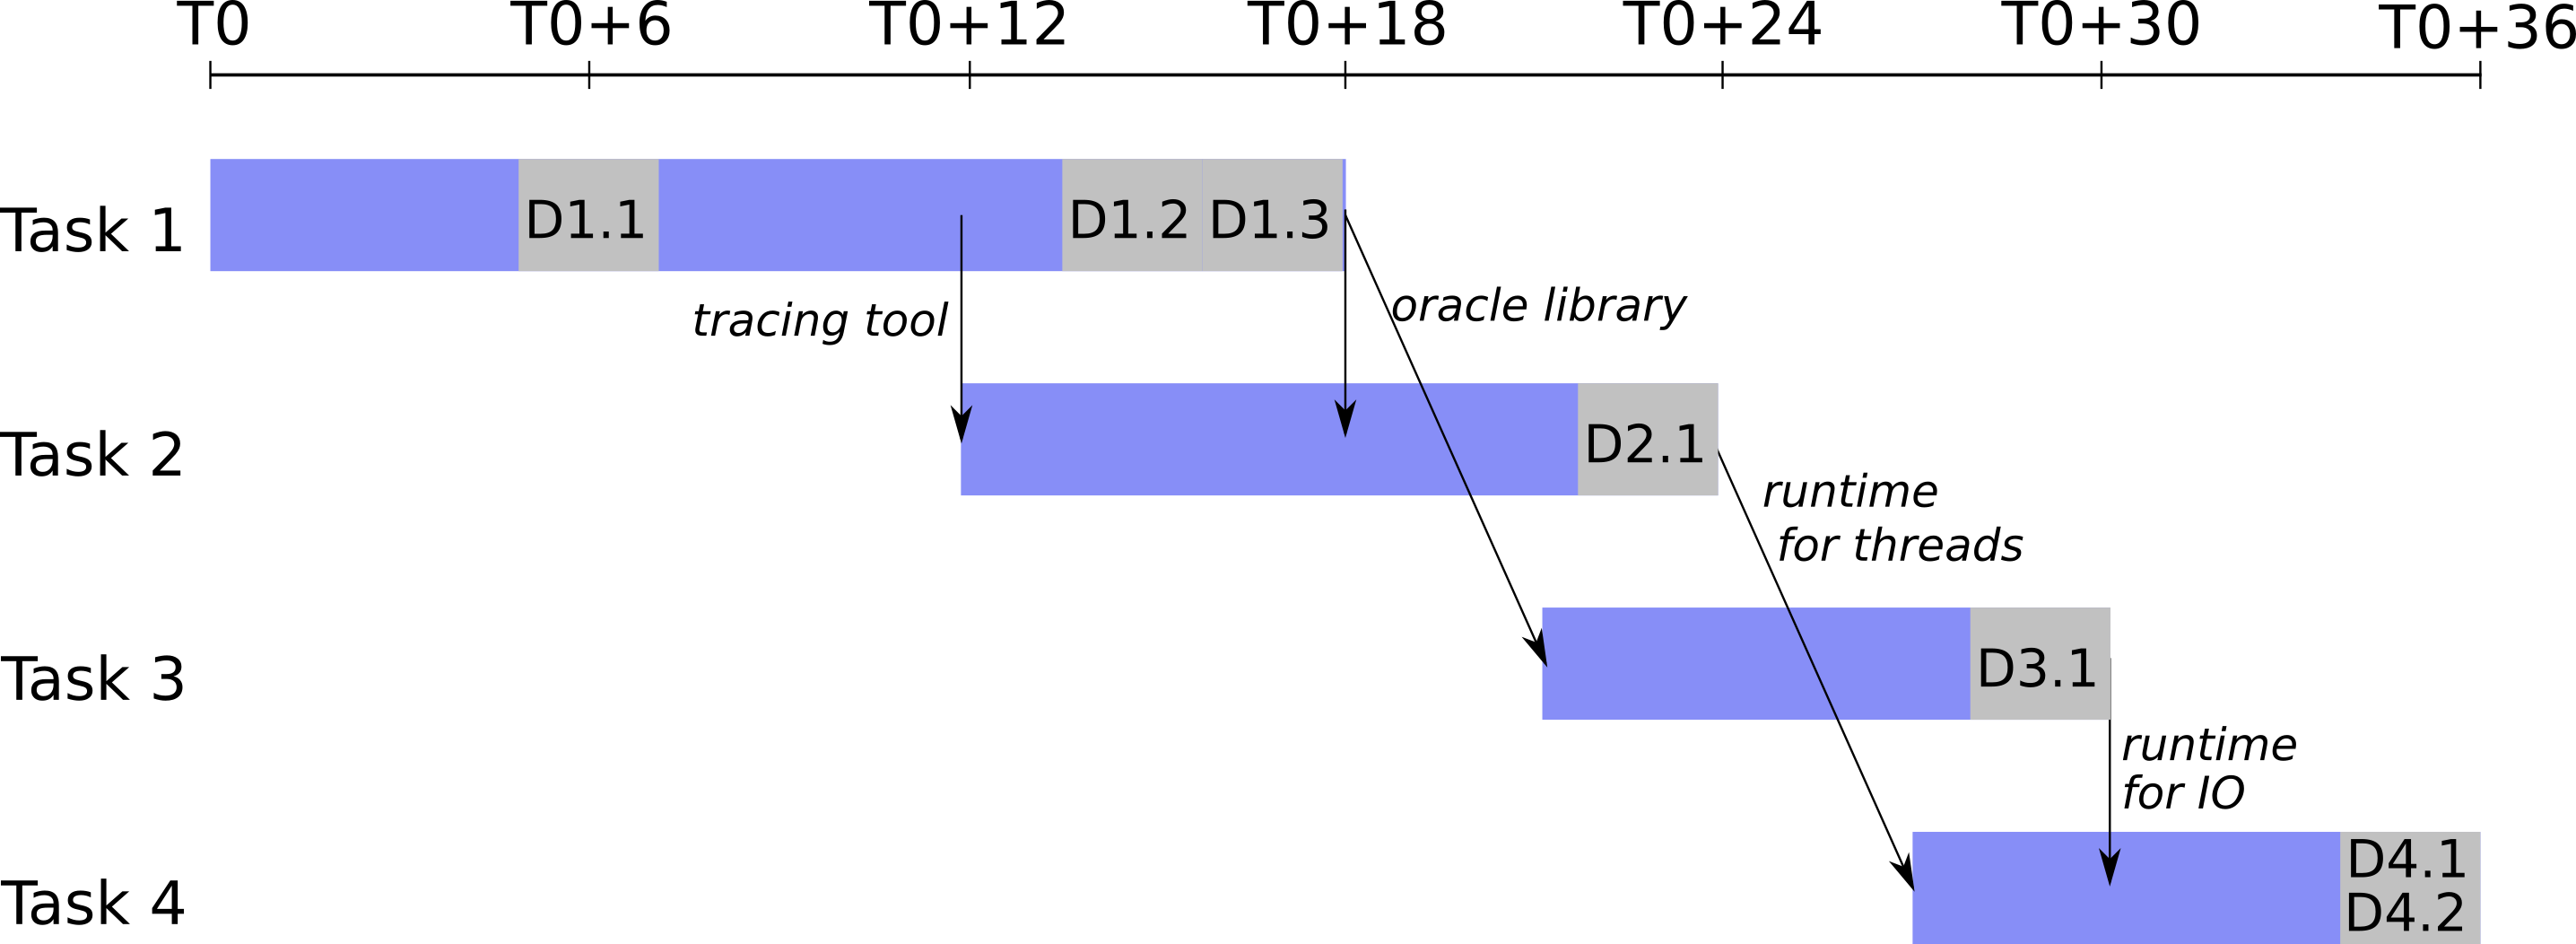
\includegraphics[width=0.8\linewidth]{figures/gantt.png}
  \caption{Gantt chart of the project}
  \label{fig:gantt}
\end{figure}

As described in the Gantt chart in Figure \ref{fig:gantt}, the \pname
project is structured in 4 main tasks:
\begin{itemize}
  \item \textbf{Task 1} will design and implement a tool-chain that
    captures the behavior of a parallel application, and generates a
    set of files that describe the captured application.
  \item \textbf{Task 2} will design and implement a runtime system for
    placing threads on a large machine. The runtime system will use
    the description files in order to predict which resource the
    threads are about to use.
  \item \textbf{Task 3} will design and implement a runtime system for
    prefetching I/O requests. It will use the description files in
    order to predict which files and data blocks are about to be used
    by the application.
  \item \textbf{Task 4} aims at evaluating the prototypes developed in
    Tasks 2 and 3 on real applications. It also aims at finalizing the
    tool-chain so that it can be used in other runtime systems.
\end{itemize}

\subsection{Description of the Tasks}
% Décrire le programme scientifique et justifier la décomposition en
% tâches du programme de travail en cohérence avec les objectifs
% poursuivis.
%  - Pour chaque tâche, décrire les objectifs, le programme détaillé des
%    travaux, les livrables, les contributions des membres de l’équipe,
%    les méthodes et les choix techniques, les risques et les solutions
%    de repli envisagées.
%
%  - Pour les projets de recherche traitant de sujets pouvant porter
%    atteinte à l’homme, aux animaux et/ou à l’environnement,
%    développer les aspects éthiques du projet.
%
%  - Illustrer par un diagramme de Gantt.
%
% Décrire les moyens mis en œuvre et demandés pour atteindre les objectifs.

%  - Justification scientifique et technique des moyens demandés par
%    grand poste de dépense et par partenaire, en lien avec les
%    objectifs de la proposition. Présenter la demande financière de
%    chaque partenaire dans le tableau « Moyens demandés par grand
%    poste de dépense et par partenaire » en veillant à la cohérence
%    de ces informations avec celles saisies sur le site de soumission
%    et à la conformité au règlement relatif aux modalités
%    d’attribution des aides de l’ANR.
%
%  - Présentation du contexte en termes de moyens humains et
%    financiers du projet au regard notamment d’autres projets en
%    cours.
%
%  - Préciser, le cas échéant, les conditions d’accès à une très
%    grande infrastructure de recherche (TGIR).

\vspace{1cm}
\subsubsection{Task 1: Extracting state automatons from a trace}
\vspace{0.5cm}
\begin{center}
    \begin{tabular} {|c|c|c|c|}\hline
      \multicolumn{4}{|l|}{\textbf{leader:} \francois }\\\hline
      Involved partners& François \textsc{Trahay}& Gaël \textsc{Thomas} & PhD student\\\hline
      Involvement& 12 & 1 & 15\\\hline
      \multicolumn{4}{|l|}{\textbf{Input:} EZTrace tracing framework, Pattern detection algorithm}\\\hline
      \multicolumn{4}{|l|}{\textbf{Output:} Oracle library}\\\hline
      \multicolumn{2}{|l|}{\textbf{Start:} $T_0$} &  \multicolumn{2}{|l|}{\textbf{End:} $T_0$+18}\\\hline\hline

      \textbf{Deadline} & \multicolumn{3}{|p{10cm}|}{\textbf{Delivrable}}\\
      T0+6& \multicolumn{3}{|p{10cm}|}{
        D1.1: A tracing library able to generate OTF2 trace files (open-source software)}\\
      
      T0+15& \multicolumn{3}{|p{10cm}|}{
        D1.2: A trace analysis tool able to detect patterns
        of events and to generate files that depict the application
        behavior (open-source software)}\\

      T0+18&\multicolumn{3}{|p{10cm}|}{D1.3: An Oracle library (open-source software)}\\\hline
    \end{tabular}
\end{center}

\begin{paragraph}{Goal:}
To extract useful information from a trace
\end{paragraph}

\begin{paragraph}{Detailed work program:}

  There are many performance analysis tools targeting various system
  components (memory management, network stack, I/O stack,
  etc.). These tools capture an application execution and provide the
  application developer with various indicators. It is then up to the
  developer to use these indicators for improving the application,
  either by modifying algorithms, or by changing the settings of the
  application (thread binding, etc.)

  The goal of this Task is to develop a tool-chain that will capture
  the behavior of an application, and generate a set of files
  describing the application. These files will be used by the runtime
  systems developed in Tasks 2 and 3 for future executions of the
  application.
\end{paragraph}

\begin{paragraph}{Task1.1: capturing the application behavior}

\begin{paragraph}{Goal:}
To run an application and capture its behavior.
\end{paragraph}

\begin{paragraph}{Detailed work program:}
  In order to analyze the performance of an application, it is crucial
  to capture its behavior without altering its execution. The overhead
  caused by the instrumentation of the application and the collect of
  traces needs to be as low as possible.

  In this Task, we will extend our existing work on the EZTrace
  tracing tool \cite{eztrace} in order to make it generate trace files
  in a standard format such as OTF2 \cite{otf2}. Since EZTrace already
  generates files in several trace formats (such as Pajé or OTF), we
  expect that the development cost will be light. However, it will
  improve the inter-operability of EZTrace with other performance
  analysis tools.

  In this Task, we will also design and implement trace analysis
  algorithms for detecting the application behavior from a trace
  file. In a previous work \cite{eztrace_pdp}, we designed a pattern
  discovery tool able to detect repetitive sequences of events
  generated by a thread in a trace. We will extend this work in
  several ways:

  \begin{itemize}
  \item We will implement a driver so that several trace formats can
    be read. This will allow the pattern discovery tool to process
    OTF2 traces generated by either EZTrace or other standard tracing
    tools (such as the Score-P suite \cite{scorep}).

  \item We will extend the pattern matching algorithm so that events
    generated by multiple threads can be compared. This would permit
    to differentiate the patterns of events that are common to
    multiple threads from those that are specific to a thread.

  \item We will extend the trace analysis tool so that it writes the
    detected behavior in a set of files that could be used for future
    execution of the application.
  \end{itemize}

\end{paragraph}

\begin{paragraph}{Delivrables:}
  \begin{itemize}
  \item[T0+6] [D1.1]: A tracing library able to generate OTF2 trace files (open-source software)
  \item[T0+15] [D1.2]: A trace analysis tool able to detect patterns
    of events and to generate files that depict the application
    behavior (open-source software)
  \end{itemize}
\end{paragraph}

\end{paragraph}                 %Task 1.1


\begin{paragraph}{Task1.2: designing an oracle library}

\begin{paragraph}{Goal:}
  To predict the future behavior of a thread.
\end{paragraph}

\begin{paragraph}{Detailed work program:}

  In this Task, we will design and implement a library that compares
  the current execution of a program and its past executions in order
  to predict the events that are likely to occur in the future. This
  library will be used in Tasks 2 and 3 for giving hints on the
  application to runtime systems.

  The library we intent to design will base its prediction on the
  files generated by the trace analyzer developed in Task 1.1. The
  behavior of an application can be viewed as a probabilistic automaton:
  given a sequence of events, the events that are likely to occur in
  the future can be predicted based on past execution of the
  application.

  The oracle library will provide an API so that runtime systems can
  inform the oracle with the events that occur. The API will also
  provide runtime systems with a way to predict the events that will
  occur in the future.

\end{paragraph}

\begin{paragraph}{Delivrables:}
  \begin{itemize}
  \item[T0+18] [D1.3]: An Oracle library (open-source software)
  \end{itemize}
\end{paragraph}

\end{paragraph}                 %Task 1.1

\begin{paragraph}{Risks and backup solutions:}
  The main risk of this task is to not be able to predict future
  events accurately.
%
  We are confident that the risk is low as in recent experiments, we
  have shown that our existing pattern detection algorithm is able to
  find repetitive sequences of events in execution traces from many
  different applications. Because applications are naturally highly
  structured, an oracle can perform predictions in any case. In a
  worst case scenario, the predictions could still be performed but a
  lower accuracy.

  Another risk is the incompatibility of the tool-chain with other
  performance analysis tools such as Score-P. The risk is low as
  EZTrace already supports several tracing format (including OTF), and
  we are confident that porting the tool-chain to OTF2 can be done. In
  case the risk materializes, we will fall back to other open trace
  formats (such as OTF or Pajé).
\end{paragraph}

%%%%%%%%%%%%%%%%%%%%%%%%%%%%%%%%%%%%%%%%%%%%%%%%%%%%%%%%%%%%%%%%%%%%%%%%


\vspace{0.5cm}
\subsubsection{Task 2: Oracle-based dynamic placement of threads}
\vspace{0.5cm}

\begin{center}
    \begin{tabular} {|c|c|c|c|c|}\hline
      \multicolumn{5}{|l|}{\textbf{leader:} \francois }\\\hline
      Involved partners& François \textsc{Trahay}& Gaël \textsc{Thomas} & PhD student & Intern\\\hline
      Involvement& 5 & 1 & 8&6\\\hline
      \multicolumn{5}{|l|}{\textbf{Participants:} Kevin \textsc{Marquet} (INSA), Lionel \textsc{Morel} (CEA)}\\\hline
      \multicolumn{5}{|l|}{\textbf{Input:} EZTrace, Oracle library (from Task 1)}\\\hline
      \multicolumn{5}{|l|}{\textbf{Output:} runtime system for thread placement}\\\hline
      \multicolumn{2}{|l|}{\textbf{Start:} $T_0$+12} &  \multicolumn{3}{|l|}{\textbf{End:} $T_0$+24}\\\hline\hline

\textbf{Deadline} & \multicolumn{4}{|p{10cm}|}{\textbf{Delivrable}}\\
      T0+24& \multicolumn{4}{|p{10cm}|}{
        D2.1: a runtime system that proactively adapts the threads placement (open-source software)}\\\hline

    \end{tabular}
\end{center}

\begin{paragraph}{Goal:}
A runtime system that dynamically places threads
\end{paragraph}

\begin{paragraph}{Detailed work program:}

  On large NUMA machines, the thread placement can significantly
  affect the performance of applications: on some applications,
  allocating memory correctly may improve the execution time by 3.6x
  relative to the default allocation strategy \cite{carrefour} ; on
  high-speed networks, a bad thread placement may degrade the
  performance by up to 40 \% \cite{nuioa}; the performance of disk I/O
  can vary by up to 33 \% depending on the thread placement
  \cite{diskio_numa}.

  In this Task, we will design a runtime system able to proactively
  adapt the placement of threads. This runtime will provide the oracle
  library developed in Task 1.2 with information on the threads usage
  of various resources (network, disk, memory, etc.) The oracle
  library can then predict the events that are likely to happen in the
  future. The runtime system can thus use the prediction in order to
  identify which resources the threads will use in the future, and to
  adapt the thread binding.

  As part of this Task, we will continue a recent collaboration with
  INSA and CEA that aims at analyzing the memory access patterns of
  parallel applications \cite{numamma}. The current work on this topic
  consists in analyzing the memory access pattern so that the
  application developer can adapt his program. In \pname, we intend to
  automate this process so as to relieve the developer from this task.

\end{paragraph}

\begin{paragraph}{Delivrables:}
  \begin{itemize}
  \item[T0+24] [D2.1]: a runtime system that proactively adapts the threads placement (open-source software)
  \end{itemize}
\end{paragraph}

\begin{paragraph}{Risks and backup solutions:}
  The main risk of this task is that the designed runtime system
  cannot improve the performance of a wide range of applications. To
  mitigate this risk, we will avoid application-specific runtime
  strategies. In case the designed strategies benefit so only some
  applications, we will analyze the evaluated applications in order to
  define the key characteristics that affect the performances of the
  runtime strategies.
\end{paragraph}


%%%%%%%%%%%%%%%%%%%%%%%%%%%%%%%%%%%%%%%%%%%%%%%%%%%%%%%%%%%%%%%%%%%%%%%%

\vspace{0.5cm}
\subsubsection{Task 3: prefetching irregular I/O}
\vspace{0.5cm}
\begin{center}
    \begin{tabular} {|c|c|c|c|}\hline
      \multicolumn{4}{|l|}{\textbf{leader:} \francois }\\\hline
      Involved partners& François \textsc{Trahay}& Gaël \textsc{Thomas} & PhD student\\\hline
      Involvement& 5 & 1 & 8\\\hline
      \multicolumn{4}{|l|}{\textbf{Participants:} Jianwei \textsc{Liao} (SWU)}\\\hline
      \multicolumn{4}{|l|}{\textbf{Input:} EZTrace, Oracle library (from Task 1)}\\\hline
      \multicolumn{4}{|l|}{\textbf{Output:} runtime system for I/O prefetching}\\\hline
      \multicolumn{2}{|l|}{\textbf{Start:} $T_0$+21} &  \multicolumn{2}{|l|}{\textbf{End:} $T_0$+30}\\\hline\hline

      \textbf{Deadline} & \multicolumn{3}{|p{10cm}|}{\textbf{Delivrable}}\\
      T0+30& \multicolumn{3}{|p{10cm}|}{
        D3.1: A runtime system that prefetches irregular I/O
    requests (open-source software)}\\\hline


    \end{tabular}
\end{center}

\begin{paragraph}{Goal:}
A runtime system that predicts future I/O requests
\end{paragraph}

\begin{paragraph}{Detailed work program:}

  Due to the huge performance difference between accessing data in
  memory and accessing data on a disk, optimizing I/O can be crucial
  for some classes of applications. Prefetching data that will be read
  in the future allows to overlap I/O operations and computation and
  can improve the overall performance. Predicting future I/O requests
  have long been studied \cite{Patterson, chang1999automatic,
    cao1996implementation}, and regular I/O access patterns can be
  predicted efficiently. However, irregular I/O access patterns are
  more difficult to predict because I/O predictors only consider the
  I/O requests previously issued in the current application
  execution. Relying on both the current execution and past executions
  would allow I/O prefetchers to predict irregular I/O access
  patterns.

  In this Task, we will design and implement a runtime system able to
  prefetch I/O data. This runtime system will use the API of the
  oracle library each time the application performs an I/O
  request. Based on these events, the oracle will provide the runtime
  system with prediction of I/O access that are likely to occur in the
  future. The runtime system may then choose to prefetch the data that
  will be accessed later.

  To pursue this Task, we will work in close collaboration with
  Jianwei \textsc{Liao} from the Southwest University (SWU) in
  China. In order to do this, we plan multiple visits, including:
  \begin{itemize}
  \item an early one week visit for François \textsc{Trahay} and the
    PhD student to SWU. This visit would initiate the collaboration on this task.
  \item a one week visit for the PhD student to SWU. During this
    visit, the PhD student would finalize the prototype, and conduct
    experiments in collaboration with Jianwei \textsc{Liao}.
  \end{itemize}

\end{paragraph}

\begin{paragraph}{Delivrables:}
  \begin{itemize}
  \item[T0+30] [D3.1]: A runtime system that prefetches irregular I/O
    requests (open-source software)
  \end{itemize}
\end{paragraph}

\begin{paragraph}{Risks and backup solutions:}
  The main risk of this task is that the proposed prefetching
  algorithm cannot improve the performance of real life
  applications. To reduce this risk, we will first study the I/O
  access patterns of several applications prior to designing the
  prefetching strategies.
\end{paragraph}


%%%%%%%%%%%%%%%%%%%%%%%%%%%%%%%%%%%%%%%%%%%%%%%%%%%%%%%%%%%%%%%%%%%%%%%%

\vspace{0.5cm}
\subsubsection{Task 4: Integration and large-scale experimental evaluation}
\vspace{0.5cm}
\begin{center}
    \begin{tabular} {|c|c|c|c|c|}\hline
      \multicolumn{5}{|l|}{\textbf{leader:} \francois }\\\hline
      Involved partners& François \textsc{Trahay}& Gaël \textsc{Thomas} & PhD student & Intern\\\hline
      Involvement& 2 & 0& 5 & 6\\\hline
      \multicolumn{5}{|p{12cm}|}{\textbf{Input:} runtime system for thread placement (from Task 2), runtime system for I/O prefetching (from Task 3)}\\\hline
      \multicolumn{5}{|l|}{\textbf{Output:} Stable version of the Oracle library}\\\hline
      \multicolumn{2}{|l|}{\textbf{Start:} $T_0$+27} &  \multicolumn{3}{|l|}{\textbf{End:} $T_0$+36}\\\hline\hline

      
      \textbf{Deadline} & \multicolumn{4}{|p{10cm}|}{\textbf{Delivrable}}\\
      T0+36& \multicolumn{4}{|p{10cm}|}{
        D4.1: Evaluation of Tasks 2 and 3 on real application (report)}\\

      T0+36& \multicolumn{4}{|p{10cm}|}{
        D4.2: A website with a trace repository}\\\hline

    \end{tabular}
\end{center}

\begin{paragraph}{Task4.1: Large-scale experimental evaluation}

\begin{paragraph}{Goal:}
To test the results of Tasks 2 and 3 on real applications.
\end{paragraph}

\begin{paragraph}{Detailed work program:}

  This task aims at evaluating the developed runtime systems and
  performance analysis tool-chain on real life applications running on
  large machines.

  As part of the development of the runtime systems in Tasks 2 and 3,
  and of the performance analysis tool-chain in Task 1, we will have
  evaluated our implementation on small applications and micro
  benchmarks. In this Task, we plan to evaluate our implementation on
  real applications running on large machines.

  This evaluation aims at assessing the scalability of the tool-chain
  developed in \pname: are the tools capable of analyzing large source
  codes ? How do they behave when running on many cores ? Can the
  oracle correctly predict future events on such application ?

\end{paragraph}

\begin{paragraph}{Delivrables:}
  \begin{itemize}
  \item[T0+36] [D4.1]: Evaluation of Tasks 2 and 3 on real application (report)
  \end{itemize}
\end{paragraph}

\end{paragraph}


\begin{paragraph}{Task4.2: Project valorisation}

  \begin{paragraph}{Goal:}
    To finalize the prototypes so that they can be used by others
  \end{paragraph}

  \begin{paragraph}{Detailed work program:}
  In this Task, we will set up facilities so that the software
  developed in \pname can be used by the research community. An effort
  will be put in stabilizing the source code of the tool-chain and
  to document the tools.

  We will also create a trace repository containing the execution
  traces gathered during \pname. The goal of this repository is to
  allow other researchers to analyze traces and to propose new
  optimization strategies.
  \end{paragraph}
  \begin{paragraph}{Delivrables:}
  \begin{itemize}
  \item[T0+36] [D4.2]: A website with a trace repository
  \end{itemize}
  \end{paragraph}

  \begin{paragraph}{Risks and backup solutions:}
There is a risk that we cannot experiment the proposed runtime systems
on actual applications. In this case, we will use mini-apps developed
for evaluating the I/O subsystem such as the one from the Virtual
Institute for I/O \footnote{https://www.vi4io.org/}. We could also
fall back to large-scale mini-apps such as the CORAL benchmark
applications \footnote{https://asc.llnl.gov/CORAL-benchmarks/}.
  \end{paragraph}

\end{paragraph}





\subsection{Task schedule, deliverable, and milestones}
We sum up the Task schedule graphically in Table
\ref{tab:task_schedule}. A synthetic view of the deliverables is
presented in Table \ref{tab:deliverables}.

% task 1: 0-18
% - task 1.1.
%    - D1.1 T+6 (tracing library)
%    - D1.2 T+15 (pattern detection)
% - task 1.2
%    - D1.3 T+18 (oracle lib)
% Task 2 : 12-24
%    - D2.1: runtime threads
% Task 3: 21-30
%    - D3.1: runtime IO
% Task 4: 27-36
%    - D4.1: eval (report)
%    - D4.2: website traces


\begin{table}[H]
  \begin{center}
    \begin{tabular} {|c|c|c|c|c|c||c|c|c|c||c|c|c|c|}
       \cline{3-14}
       \multicolumn{2}{c|}{}    & \multicolumn{4}{|l|}{Year 1 } &\multicolumn{4}{|l|}{Year 2 } & \multicolumn{4}{|l|}{Year 3}\\
              \cline{3-14}
       \multicolumn{2}{c|}{}  & 3 & 6 & 9 & 12 & 15 & 18 & 21 & 24 & 27 & 30 & 33 & 36\\\hline
      \multirow{2}{*}{ Task 1} & Subtask 1.1 & \task & \task \delsoft & \task & \task & \task \delsoft &  &  &  &  &  &  & \\
      & Subtask 1.2 & & \task & \task & \task & \task & \task \delsoft &  &  &  &  &  & \\\hline\hline
      \multicolumn{2}{|l|}{Task 2} & &  &  & & \task & \task & \task & \task \delsoft &  &  &  & \\\hline\hline
      \multicolumn{2}{|l|}{Task 3} & &  &  &  &  &  &  & \task & \task & \task \delsoft &  & \\\hline\hline
      \multirow{2}{*}{Task 4} & Subtask 4.1 & &  &  &  &  &  &  & & & \task & \task &\task \delreport\\
      & Subtask 4.2 & &  &  &  &  &  &  & & & \task & \task &\task \delsoft\\\hline\hline
      \multicolumn{2}{|l|}{Progress report/Expenses} & &  &  &  &  & \progress \delexpense&  & & & &  &\progress \delexpense \\\hline
    \end{tabular}

    \begin{tabular}{c l c l c l}\\
      \multicolumn{6}{c}{Legend:}\\
      \task \delsoft & Deliverable is a software & \task \delreport & Deliverable is a report & \progress \delexpense & Progress report + expense summary
    \end{tabular}
  \end{center}
  \caption{Task schedule for \pname}
  \label{tab:task_schedule}
\end{table}


\begin{table}[H]
  \begin{center}
    \begin{tabular} {|c|p{12cm}|c|}\hline

\cellcolor{Tan}\textbf{Task} & \cellcolor{Tan}\textbf{Title and substance of the deliverable and milestone} & \cellcolor{Tan}\textbf{Delivery}\\\hline

      \multicolumn{3}{|c|}{\cellcolor{NavyBlue}\textbf{T1: Extracting state automatons from a trace}  }\\\hline
      \multicolumn{3}{|l|}{T1.1: capturing the application behavior  }\\\hline
      D1.1& A tracing library able to generate OTF2 trace files (open-source software) & T0+6\\
      D1.2& A trace analysis tool able to detect patterns
 of events and to generate files that depict the application
 behavior (open-source software) & T0+15\\\hline\hline

 \multicolumn{3}{|l|}{T1.2: designing an oracle library  }\\\hline
 D1.3&An Oracle library (open-source software)&T0+18\\\hline\hline

 \multicolumn{3}{|c|}{\cellcolor{NavyBlue}\textbf{T2: Oracle-based dynamic placement of threads}  } \\\hline
D2.1 & a runtime system that proactively adapts the threads placement& T0+24\\\hline\hline
\multicolumn{3}{|c|}{\cellcolor{NavyBlue}\textbf{T3: prefetching irregular I/O}  }\\\hline
D3.1& A runtime system that prefetches irregular I/O
    requests (open-source software) & T0+30\\\hline\hline

    \multicolumn{3}{|c|}{\cellcolor{NavyBlue}\textbf{T4: Integration and large-scale experimental evaluation}  } \\\hline
    \multicolumn{3}{|l|}{T4.1: Large-scale experimental evaluation }\\\hline
    D4.1& Evaluation of Tasks 2 and 3 on real application (report) &   T0+36\\\hline\hline
    \multicolumn{3}{|l|}{T4.2: Project valorisation  }\\\hline

 D4.2 & A website with a trace repository &   T0+36\\\hline

    \end{tabular}
  \end{center}
  \caption{Deliverables and Milestones for \pname}
  \label{tab:deliverables}
\end{table}

\subsection{Requested resources}
% Les montants indiqués dans ce tableau devront être rigoureusement
% identiques à ceux saisis sur le site de soumission de l’ANR. Si ces
% deux sources d’informations s’avéraient non concordantes, y compris
% si elles étaient mal renseignées ou manquantes, les informations
% saisies en ligne prévaudront sur celles développées dans le
% formulaire de soumission/document scientifique.
\vspace{1cm}
\subsubsection{Cost supported by ANR proposal}
\begin{paragraph}{Staff}
Two interns (master-level, 6 months) will be hired for the project (on
the 12th month, and on the 30th month) as well as a PhD student (36
months).

The PhD student will work on the design and implementation of the
oracle library, as well as on the design of the runtime systems that
exploit the oracle predictions.

The first research intern will contribute to Task 2. He/she will work
on thread scheduling strategies that take into account the future
behavior of threads. The intern will work in close relationship with
the PhD student.% \todo{a ameliorer: quel est le role du thesard vs du stagiaire ?}

The second intern will contribute to Task 4. He/she will help the PhD
student running experiments on real life applications. The intern will
also contribute to the valorisation of the software developed in
\pname by stabilizing the code, writing documentation, and deploying a
data repository where experimental results (such as trace files) will
be publicly available.
\end{paragraph}

\begin{paragraph}{Mission, traveling, and workshop}
  % total: 25k
  % - conf: 9
  % - conf euro: 6
  % - chine:  9k
  % - workshop: 1k
  The traveling costs are evaluated as follows:
  \begin{itemize}
  \item Attending one international conference for one member of the
    project during 3 years. \emph{Cost: 3 x 3k\euro = 9 k\euro}
  \item Attending one european conference for one member of the
    project during 3 years. \emph{Cost: 3 x 2k\euro = 6 k\euro}
  \item Three one-week visits to our partner in China as part of Task
    2. \emph{Cost: 3 x 3 k\euro = 9 k\euro}
  \end{itemize}

  Finally, we plan to organize a one-day workshop around performance
  analysis in conjunction with a major national conference at the end
  of the 2nd year of the project. The cost (food and breaks) will be
  partly supported by ANR (20 people): 1000 \euro.
\end{paragraph}

\begin{paragraph}{Hardware \& Inward billing}
  Two laptops will be bought for members of the project. \emph{Cost: 2 x 2.5 k\euro}

  In order to run experiments on a large scale machine, we will buy a
  large NUMA machine able to run 192 threads. According to a
  quotation, such machine would cost approximately 25 k\euro.
\end{paragraph}

\vspace{0.3cm}
\subsubsection{Cost not supported by ANR proposal}
\begin{paragraph}{Permanent staff}

  Dr. François \textsc{Trahay}, the principal investor of \pname, will
  spend 66 \% of his time (24 p.m) working on the project. In addition
  to supervising the PhD student and the interns, he will participate
  to the design and development of the software.

  Prof. Gaël \textsc{Thomas} will spend 3 p.m working on the
  project. He will help supervising the PhD student, and will help
  designing the tools to be developed in the project.

\end{paragraph}

% For this project, we ask for 168k{\euro}. Included in this budget
%   are: a PhD student ($\sim$ 110k\euro) , a large (100+ cores) NUMA
%   machine for running experiments ($\sim$ 30k\euro),
%   two annual trips to conferences for two researchers ($\sim$
%   20k\euro), and the funding for organizing two workshops ($\sim$
%   8k\euro).
%
%   \todo{Ajouter:
%     - 1 visite de 1 semaine pour 2 en chine (4k)
%     - 1 visite de 1 semaine pour 1 en Chine (2k)
%   }
\vspace{0.3cm}
\subsubsection{Summary of the project cost}

\begin{center}
%\begin{scriptsize}
  \begin{tabular} {|l|c|c|}\hline
    & Cost & Requested funding\\\hline
    Permanent staff / \emph{Frais de personnel permanents}                      & 199 k\euro & 0\\\hline
    Staff / \emph{Frais de personnel}                      & 122 k\euro & 122 k\euro\\\hline %(1 phd+ 12 month intern)
Hardware / \emph{Coûts des instruments et du matériel} & 30 k\euro &30 k\euro\\\hline % (25k NUMA + 5k laptops)
%\emph{Coûts des bâtiments et des terrains}             &  0 &0\\\hline
%\emph{Prestation de service et droits de propriété intellectuelle}& 0&0\\\hline
Travel / \emph{Missions}                               & 25 k\euro&25 k\euro\\\hline
Administrative fees / \emph{Frais d’environnement}     & 14 k\euro&14 k\euro \\\hline
\textbf{Sub-total} / \emph{Sous-total}                 & \textbf{389 k\euro}& \textbf{191 k\euro}\\\hline
\textbf{Requested funding} / \emph{Aide demandée}      & - &\textbf{191 k\euro}\\\hline
\end{tabular}
%\end{scriptsize}
\end{center}

% \todo{mettre a jour le budget. On veut tenir dans 180ke
%   \begin{itemize}
%   \item staff: 125k (phd+intern)
%   \item matos: 30k (numa: 25k + 2 laptop=5k)
%   \item mission: 15k
%   \item frais d'environnement: 8\% * 170=13.6ke
%   \item total: 183.6ke
%   \end{itemize}
% }

%  Pour les Bénéficiaires à coût marginal, ces frais correspondent à
%  un forfait de 8% des dépenses éligibles (hors frais
%  d’environnement), dans la limite du plafond d’Aide accordé. Pour
%  les Bénéficiaires à coût complet, ces frais sont calculés : d’une
%  part, sur les dépenses de personnels et plafonnés pour cette part à
%  68% des dépenses de personnel ; d’autre part, sur les dépenses
%  autres que de personnels, pour cette part à 7% des dépenses (hors
%  frais d’environnement).


% \subsubsection{Cost not supported by ANR proposal}
% 
% \begin{paragraph}{Experimental resources}
%   We will run the experiments of \pname on several existing platforms:
%   \begin{itemize}
%   \item We will use the hardware resources provided by the Grid5000
%     platform
% 
%   \end{itemize}
% \end{paragraph}


\subsection{Consortium around \pname}
% - Présenter le coordinateur scientifique et son implication dans le
%   projet et son positionnement au sein de son organisme ou
%   laboratoire d’accueil
% - Présenter l’équipe constituée autour du projet objet de la
%   proposition, sa qualité, sa complémentarité
\vspace{0.8cm}
\subsubsection{Scientific leader}
The Principal Investigator of the \pname project is François
\textsc{Trahay}. He will devote sixty-six percent of his research time to
the project.  François \textsc{Trahay} is an associate professor at
Télécom SudParis (TSP) since 2011.
%
He is a member of the HP2 team of the computer science
department, which investigates high-performance systems.
%
He received his Ph.D. degree in computer science from the University
of Bordeaux in 2009. He has been working on runtime systems for high
performance computing since 2006. His research interests now mostly
focus on performance analysis for HPC and distributed systems. He is
the project leader and main developper of the EZTrace framework for
performance analysis.
%
He is the co-author of 19 research papers in top international
conferences, workshops and journals such as IEEE TPDS, IPDPS, ICPP,
IEEE Cluster, ACM TACO, or IJPP.
\vspace{0.3cm}
\subsubsection{Scientific environment}
% présenter l'équipe
In addition to the principal investigator, the project will involve
the HP2 team at Télécom SudParis. HP2 is composed of experts in
runtime systems for high-performance computing (Dr. {\'E}lisabeth
\textsc{Brunet}, and Dr. Amina \textsc{Guermouche}), and for operating
systems (Prof. Gaël \textsc{Thomas}). Gaël \textsc{Thomas} will help
supervising the PhD student hired for this project.

\pname will also involve Dr. Jianwei \textsc{Liao} at the Southwest
University of China. He is an expert on distributed filesystems.  We
started working together on prefetching for distributed filesystems in
2015. We will work in close collaboration with Dr. \textsc{Liao} in
order to benefit from his expertise in filesystems. As part of Task 2,
we plan several trips to the Southwest University of China.
\vspace{0.3cm}

\section{Project impact, dissemination}
% Décrire la stratégie de diffusion / de valorisation envisagée.

% Décrire en quoi les attendus du projet répondent aux enjeux de
% recherche inscrits au Plan d’Action 2018

% Décrire dans quel(s) domaine(s) (scientifique, économique, social ou
% culturel) les résultats du projet peuvent avoir un impact

% S’il s’agit d’un projet Jeune chercheure-Jeune chercheur (JCJC),
% Montrer la capacité du projet à favoriser le développement d’une
% thématique ou d’une équipe propre à la jeune chercheure ou au jeune
% chercheur.

\subsection{Impact of the proposal}

In the short term, we expect that the result of the \pname project
will impact most HPC applications as the problematics of locality and
I/O overhead is commonplace.
%
Furthermore, this project addresses several challenges (scheduling,
I/O, auto-tuning, etc. ) from the Challenges of Exascale Computing
\cite{exascale_challenges}.

In the long-term, we expect that the \pname project will change the
way runtime systems are designed, and the tool-chain will be used for
other runtime decisions. We also expect that the outcomes of \pname
could be generalized and applied to other domains. During the project,
we will focus on performance improvement, but the collaboration
between a performance analysis tool and a runtime system could also be
used for reducing the energy consumption without degrading the
performance. We also expect that the results of \pname could be
transferred to big-data applications as they have similar properties
as HPC applications.


\subsection{Positionning with respect to the call}
% Décrire en quoi les attendus du projet répondent aux enjeux d’un
% (axe de) défi du Plan d’Action 2017 de l’ANR, de la SNR, de la
% recherche fondamentale

This project mainly addresses the ``Défi 7 > Axe 2 > Science et
Technologies logicielles'' challenge. Indeed, \pname will design
mechanisms that allow runtime systems to take better decisions. While
the two example runtimes that will be designed will focus on
performance of HPC applications, we expect that the mechanisms
provided by \pname could be used to other domains (eg. big data) and
to other means (eg. reducing energy consumption).
%
\pname will also address several \emph{Technical Research Priorities}
from the ETP4HPC Strategic Research Agenda \cite{etp4hpc} including priority
\#2 System software and management, and priority \#3 programming
environment.

% results: an open-source tool chain for performance analysis
% science: new data mining methods for performance analysis
% 

% As primary use cases, the Swipe project will study applications from
% three emerging domains that are of prime importance for France and
% Europe: (i) Neuroimaging, a core research and medical priority; (ii)
% Biometrics, a key technological field for the management of numerical
% identity, improvement of border control security solutions,
% development of law enforcement capabilities to detect and analyze
% organized crime trends; (iii) Large-scale cloud storage, a field of
% major economic importance, which is also related to technical
% sovereignty issues for citizens and businesses.

\subsection{Valorization strategies, dissemination, and exploitation of results}

\begin{paragraph}{Software}
The investigator of the project will continue his commitment to
open-source as all the tools developed during the
project will be freely available as open-source software.
%
Besides, the software will be maintained beyond the end of
the project and efforts will be made to bootstrap a visible and
active community of users and contributors, through appropriate
channels and organizations.

In addition to software, we also plan to make our research results
freely available. We will create a data repository where experiment
results such as execution traces, and experiment configuration (eg. a
docker file for running the experiment, information on the machine
topology, etc.) will be available.
\end{paragraph}


\begin{paragraph}{Collaboration}
  We expect that the outcomes of the project will trigger collaborations
  or enforce existing ones. \pname could be used as part of the new
  collaborations that we started with INSA Lyon and CEA.
  %
  Moreover, François Trahay already worked on parallel I/O
  \cite{prefetch_liao} with researchers from the Southwest University in
  Chongqing (China). \pname could be used for continuing such
  international collaborations.

  François Trahay recently initiated a collaboration with DDN, the
  leading company on I/O architectures for HPC. This collaboration has
  led us to propose a FUI project that aims at transferring research
  results (including parts of the EZTrace tracing tool) to industrial
  partners like DDN, Criteo, or Qarnot computing. We intend to
  continue this collaboration and to develop new ones. We expect that
  the results of \pname (for instance, the runtime system for I/O
  prefetching) could be part of a supplementary relationship with DDN.
\end{paragraph}

\begin{paragraph}{Publication}
  During the project, we intend to publish the scientific results.
  These results will be published in major international conferences
  (such as IPDPS, EuroPar, ICPP, ASPLOS, SOSP, etc.) and journals
  (TPDS, IJPP, etc.) We also intend to disseminate scientific results
  to the french community as part of the Compas conference. \todo{a
    garder ?}
\end{paragraph}

\subsection{Reproductibility}

The ability to reproduce research results is a growing
concern. \pname will contribute to this effort in several ways:
\begin{itemize}
\item All the tools developed as part of this ANR project will be freely available as open-source ;
\item We will create a data repository where the experiment results
  (for instance, the execution traces), as well as the software
  configuration (eg. docker file for running the experiment) will be
  available.
\end{itemize}

We believe that such data and source repositories will help the
research community reproduce research results, and propose new
performance analysis algorithms or runtime system strategies.


%\section{Bibliography}

\bibliographystyle{IEEEtran}
\bibliography{main}{}


%\end{thebibliography}
\end{document}

%% Local Variables:
%% TeX-master: "main.tex"
%% ispell-dictionary: "en_US"
%% mode: latex
%% mode: flyspell
%% coding: utf-8
%% End:
